\documentclass{article}
\linespread{1.3}
\usepackage[margin=50pt, headheight=60pt, headsep=0pt]{geometry}
\usepackage{amsmath, amssymb, amsthm, tikz, fancyhdr, float, graphicx, spverbatim, systeme}
\pagestyle{fancy}
\renewcommand{\headrulewidth}{0pt}
\newcommand{\changefont}{\fontsize{15}{15}\selectfont}

\fancypagestyle{firstpageheader}{
  \fancyhead[R]{
    \changefont
    \parbox[t]{4cm}{ % Adjust width as needed
      Michael Huang\\
      EN.625.740.81\\
      Homework 9
    }
  }
}

\begin{document}

\thispagestyle{firstpageheader}
{\Large 

\section*{1.}
Show a perceptron that calculates \(\bar{x}_1 x_2 \bar{x}_3\). \\ \\
This is essentially NOT \(x_1\) AND \(x_2\) AND NOT \(x_3\). We aim to have a target end state where we only get a positive value when \(x_2\) is positive. An easy way to guarantee this is to have a positive coefficent for \(x_2\) and negative for the other two. Summing this gives us something like \(-x_1 + x_2 - x_3\) which we can easily see will be equal to or below 0 when any of \(x_1\) or \(x_3\) are true / 1. The only remaining cases are now when both are false / 0. When \(x_2\) is also false or 0 in this case, then we indeed get 1 when \(x_2\) is true / 1, and 0 otherwise. So in this case, with \(s(a)\) being the function from the text where it gives 1 if \(a \geq 0\), we therefore need to adjust this accordingly with to ensure that these are all below 0 in all other cases, so we can set our bias to -0.5 to ensure all outputs are below 0 except for the target case. Therefore:
\[
  \boxed{y = s(-x_1 + x_2 - x_3 - 0.5)}
\]

}
{\Large 

\section*{2.}
Show a perceptron that calculates \(\bar{x}_2 x_3\). \\ \\
This is essentially NOT \(x_2\) AND \(x_3\). We aim to have a target end state of 1 only when \(x_2\) is false / 0 and \(x_3\) is true / 1. Looking case by case, we can approach this similarly to the previous problem, with penalizing \(x_2\) being true / 1 by setting it to a negative coefficient, and the opposite for \(x_3\). This is \(-x_2 + x_3\). The only case we need to account for now is that when the two are not the same value. When \(x_2\) is 0 and \(x_3\) is 1, we get 1, which is good, but when \(x_2\) is 1 and \(x_3\) is 0, we aim to get something below 0, but instead get 0. We therefore also add a bias of -0.5 here to ensure that our target case is above 0 and all other cases are below 0. Therefore:
\[
  \boxed{y = s(-x_2 + x_3 - 0.5)}
\]

}
{\Large 

\section*{3.}
Show a neural network that calculates \(\bar{x}_1 \bar{x}_2 \bar{x}_3 + x_1 x_2 x_3\). \\ \\
We basically aim to create a multi-layer perceptron that basically takes the ANDs of all NOT of the \(x\) values and all ANDs of all of the \(x\) values, and then takes the OR of these two values and gives value greater than 0 according to if either of these are 1. We can kind of reverse-engineer this -- the only case in which OR gives a nonnegative value is if the hidden layers \(z_1\) and \(z_2\) both are 0, and above 0 otherwise. So we need to keep both coefficients positive. This gives us \(z_1 + z_2\), which we see will give us 0 if both are 0. We can add the corresponding bias of -0.5 accordingly which also ensures that if either hidden layer value is 1, it will still be at least 0.5. Now looking at each layer: \\ \\
\(\bar{x_1} \bar{x_2} \bar{x_3}\), so we only get a value of above 0 when all are 0s, and negative otherwise. The easiest way to set this up is to set all coefficients to negative, which covers any of the values being 1 giving us a negative value, which ultimately outputs 0. Finally, handling all the 0s, we need to make sure this is above 0, so we add 0.5 as the bias. So we have 
\[
  \boxed{z_1 = s(-x_1 - x_2 - x_3 + 0.5)}
\] \\
\(x_1 x_2 x_3\), so we only get a value above 0 when we have all 1s. An easier way to look at this is that if we have 2 or fewer trues, then we should have a negative result. So we can see that the bias should be -2.5, since this would guarantee a positive result for all 3 trues / 1s but negative for any other, giving us 
\[
  \boxed{z_2 = s(x_1 + x_2 + x_3 - 2.5)}
\]
Finally, we combine this accordingly:
\[
  \boxed{y = s(z_1 + z_2 - 0.5)}
\]

}
{\Large 

\section*{4.}
Show a neural network that calculates \(\bar{p}_1 + x_1 x_2 x_3\). \\ \\
\(p_1\) represents the parity function of just \(x_1\). The parity of \(n\) bits is 1 if an odd number of the inputs are 1, and 0 otherwise, so \(\bar{p}_1\) simplifies directly to \(\bar{x}_1\). This simplifies the problem down to a multi-layer perceptron that takes the NOT of \(x_1\) and the AND of all of the \(x\) values, and then takes the OR of these two values. This OR is the same as the previous problem, so we have the same interaction with the the hidden layers \(z_1\) and \(z_2\); again this gives us \(z_1 + z_2\), which we see will give us 0 if both are 0; again we add the corresponding bias of -0.5. Now looking at each layer: \\ \\
\(\bar{p}_1\) is just \(\bar{x}_1\), so we only get a value of above 0 when \(x_1\) is 0, and negative otherwise. The easiest way to set this up by setting the \(x_1\) coefficient to a negative coefficient, which covers \(x_1\) being 1 which gives us a negative value. Finally, to handle the 0, we need to make sure this is above 0, so we add 0.5 as the bias, which ensures that the \(x_1 = 1\) case is still negative. So we have 
\[
  \boxed{z_1 = s(-x_1 + 0.5)}
\] \\
\(x_1 x_2 x_3\), the same as we previously calculated: 
\[
  \boxed{z_2 = s(x_1 + x_2 + x_3 - 2.5)}
\]
Finally, we combine this accordingly:
\[
  \boxed{y = s(z_1 + z_2 - 0.5)}
\]

}
{\Large 

\section*{5.}
Show a neural network that calculates \(p_2(x_1, x_2) \cdot p_3(x_1, x_2, x_3)\). \\ \\
We can start by trying to simplify the parity functions. The total product of the two parity functions must be 1, so they both must come out to 1. \(p_2\) requires exactly one of \(x_1\) or \(x_2\) to be 1 for this to be 1. \(p_3\) requires an odd number of total 1s across all three inputs (so either 1 or 3 1s). Taking this into account with the inputs, if exactly one of \(x_1\) or \(x_2\) is true / 1, then \(x_3\) must be 0 to keep the total count of 1s odd (otherwise we'll have 2 1s). Therefore, the only two input states that satisfy both conditions simultaneously are \((0, 1, 0)\) and \((1, 0, 0)\). So we can reinterpret this expression as an OR statement now, since either of these will give us the target value of 1. So we can express this as \(\bar{x}_1 x_2 \bar{x}_3 + x_1 \bar{x}_2 \bar{x}_3\). \\ \\
As we did previously, we'll create a multi-layer perceptron that calculates the hidden layers; we do the same reverse-engineering as before, with the only case in which OR gives a nonnegative value is if the hidden layers \(z_1\) and \(z_2\) both are 0, and above 0 otherwise. We again keep both coefficients positive, giving us \(z_1 + z_2\), which gives us 0 if both are 0; we can add the corresponding bias of -0.5 accordingly which also ensures that if either hidden layer value is 1, it will still be at least 0.5. Now looking at each layer: \\ \\
\(\bar{x}_1 x_2 \bar{x}_3\). We only get a value above 0 when \(x_2\) is 1 and the others are 0, and negative otherwise. We do the same thing we did in Problem 1: we set the \(x_2\) coefficient to positive (+1), and the \(x_1\) and \(x_3\) coefficients to negative (-1). Again, we want a positive result only for this exact combination, so we add -0.5 as the bias to ensure this is the case. So we have 
\[
  \boxed{z_1 = s(-x_1 + x_2 - x_3 - 0.5)}
\] \\
\(x_1 \bar{x}_2 \bar{x}_3\). This is similar to the above, but we only get a value above 0 when \(x_1\) is 1 and the others are 0. Similarly, we simply set the \(x_1\) coefficient to positive (+1), and the \(x_2\) and \(x_3\) coefficients to negative (-1). Applying the same logic for the bias, we add -0.5, giving us 
\[
  \boxed{z_2 = s(x_1 - x_2 - x_3 - 0.5)}
\]
Finally, we combine this accordingly:
\[
  \boxed{y = s(z_1 + z_2 - 0.5)}
\]

}
{\Large 

\section*{6.}
Generate two-dimensional samples for each of two Gaussians, $p(\mathbf{x}|\omega_i) \sim N(\boldsymbol{\mu}_i, \Sigma_i)$ with
\[
  \boldsymbol{\mu}_1 = \begin{pmatrix} 1 \\ -1 \end{pmatrix}, \boldsymbol{\mu}_2 = \begin{pmatrix} 0 \\ 0 \end{pmatrix}, \Sigma_1 = \begin{pmatrix} 0.2 & 0 \\ 0 & 0.2 \end{pmatrix} = \Sigma_2.
\]  
Produce 100 samples from each distribution, but to guarantee linear separability, produce a replacement for a Class 1 vector whenever \(x_1 - x_2 < 1\) and produce a replacement for a Class 2 vector whenever \(x_1 - x_2 > 1\). \\ \\
Use these vectors to design a linear classifier using the perceptron algorithm. After convergence, draw the decision boundary. 
\begin{figure}[h!]
  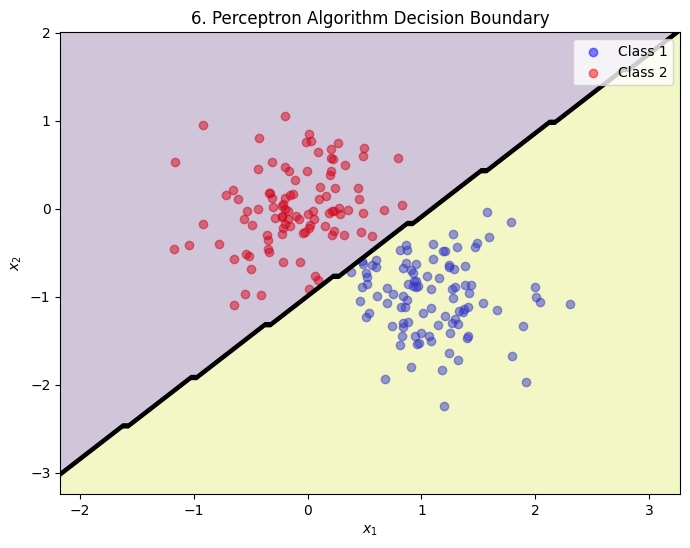
\includegraphics[width=430pt]{problem_6_perceptron_plot.png}
\end{figure}

This was the code I ran to create the above diagram:
\begin{spverbatim}
import numpy as np
import matplotlib.pyplot as plt
from sklearn.linear_model import Perceptron

mu_1 = np.array([1, -1])
mu_2 = np.array([0, 0])

cov = np.array([
  [0.2, 0], [0, 0.2]
])

class_1_samples = []
while len(class_1_samples) < 100:
  sample = np.random.multivariate_normal(mu_1, cov)
  # Reject if x_1 - x_2 < 1
  if sample[0] - sample[1] >= 1:
    class_1_samples.append(sample)
class_1_samples = np.array(class_1_samples)

class_2_samples = []
while len(class_2_samples) < 100:
  sample = np.random.multivariate_normal(mu_2, cov)
  # Reject if x_1 - x_2 > 1
  if sample[0] - sample[1] <= 1:
    class_2_samples.append(sample)
class_2_samples = np.array(class_2_samples)

# Create 200 x 2 matrix of samples + class labels
x = np.vstack((class_1_samples, class_2_samples))
y = np.hstack((np.ones(100), np.zeros(100)))

# Train linear classifier using the Perceptron algorithm
linear_classifier = Perceptron(max_iter=1000, tol=1e-5)
linear_classifier.fit(x, y)

plt.figure(figsize=(8, 6))

# Create meshgrid for plotting decision boundary
x_min, x_max = x[:, 0].min() - 1, x[:, 0].max() + 1
y_min, y_max = x[:, 1].min() - 1, x[:, 1].max() + 1
xx, yy = np.meshgrid(np.arange(x_min, x_max, 0.05),
                     np.arange(y_min, y_max, 0.05))

# Predict across the meshgrid
z_linear = linear_classifier.predict(np.c_[xx.ravel(), yy.ravel()])
z_linear = z_linear.reshape(xx.shape)

# Plot points with decision boundary regions
plt.scatter(class_1_samples[:, 0], class_1_samples[:, 1], color='blue', label="Class 1", alpha=0.5)
plt.scatter(class_2_samples[:, 0], class_2_samples[:, 1], color='red', label="Class 2", alpha=0.5)

plt.contourf(xx, yy, z_linear, alpha=0.25)
plt.contour(xx, yy, z_linear, colors="black", linewidths=1)

plt.title("6. Perceptron Algorithm Decision Boundary")
plt.xlabel("$x_1$")
plt.ylabel("$x_2$")
plt.legend()
plt.savefig("problem_6_perceptron_plot.png", bbox_inches="tight")
plt.show()
plt.close()
\end{spverbatim}

}

\end{document}